\chapter{Methodology}\label{cha: Methodology}

\section{Initial growth of a-Si and SiO\texorpdfstring{$_{2}$}{2} thin films via electron beam evaporation}\label{sec: growth}
Glass slides and Si wafers were used as substrates for the initial growth via electron beam evaporation of a-Si and SiO$_2$ thin films respectively. The substrates were cleaned by sonication in acetone, isopropanol, and deionized water for 5 minutes each, after which they were blow-dried with nitrogen gas. The substrates were then loaded into the ULVAC electron beam evaporation chamber, where a base pressure of $\qty{4.5e-4}{\Pa}$ was achieved before actual deposition. Deposition was carried out at room temperature, and the nominal deposition rates and thicknesses of the films were monitored using a \gls{QCM} with the input values in~\ref{tab: qcm_input}. 

\section{Characterization of a-Si and SiO\texorpdfstring{$_{2}$}{2} thin films}\label{sec: analysis}
After unloading the samples from the chamber, the thicknesses of the films were measured using \gls{XRR} with a Malvern Panalytical Empyrean x-ray diffractometer. Curve fitting was performed on selected samples to obtain the densities and interface roughness of the films. The refractive index of the a-Si film was determined using Swanepoel's method via UV-Vis spectroscopy with a Shimadzu UV-Vis spectrophotometer while the refractive index of the SiO$_2$ film was identified using the interference method via the reflectance spectroscopy setup as shown in~\ref{fig: magnetron}. The measured refractive indices of the a-Si and SiO$_2$ films were used for the design of the a-Si/SiO$_2$ ARC stack.

\section{Simulation and growth of a-Si/SiO\texorpdfstring{$_{2}$}{2} antireflective coatings}\label{sec: growth_and_simulation}
A \gls{TMM} implementation in Python was used to calculate the optimal thicknesses of the Si and SiO$_2$ layers for the antireflective coating stack. The refractive indices of the a-Si and SiO$_2$ layers used for the simulation were obtained from the previous section. The optimal thicknesses of the layers were calculated to minimize the reflectance at $\qty{1550}{\nano\meter}$ and $\qty{780}{\nano\meter}$, which are the wavelengths of the lasers which can be used in the THz-TDS spectroscopy system. The program iterated over a range of thicknesses for each layer while calculating the reflectance of the stack, selecting the thicknesses that resulted in the lowest reflectance at the target wavelengths. The thicknesses obtained from the simulation were then used for the growth of the a-Si/SiO$_2$ \gls{ARC} on bare wafers via electron beam evaporation. The reflectance of the samples with the antireflective coating was measured via reflectance spectroscopy and compared to the simulated reflectance to verify the accuracy of the simulation and growth process.

\begin{table}[tbp]
\centering
\begin{tabular}{lll}
\toprule
     & z-factor & $\rho$ \unit{\gram\per\cubic\centi\meter}\\
\midrule
Si   & 0.712   & 2.32 \\
SiO$_2$ & 1   & 2.65 \\
\bottomrule
\end{tabular}
\caption{QCM inputs}\label{tab: qcm_input}
\end{table}

\begin{figure}
	\centering
	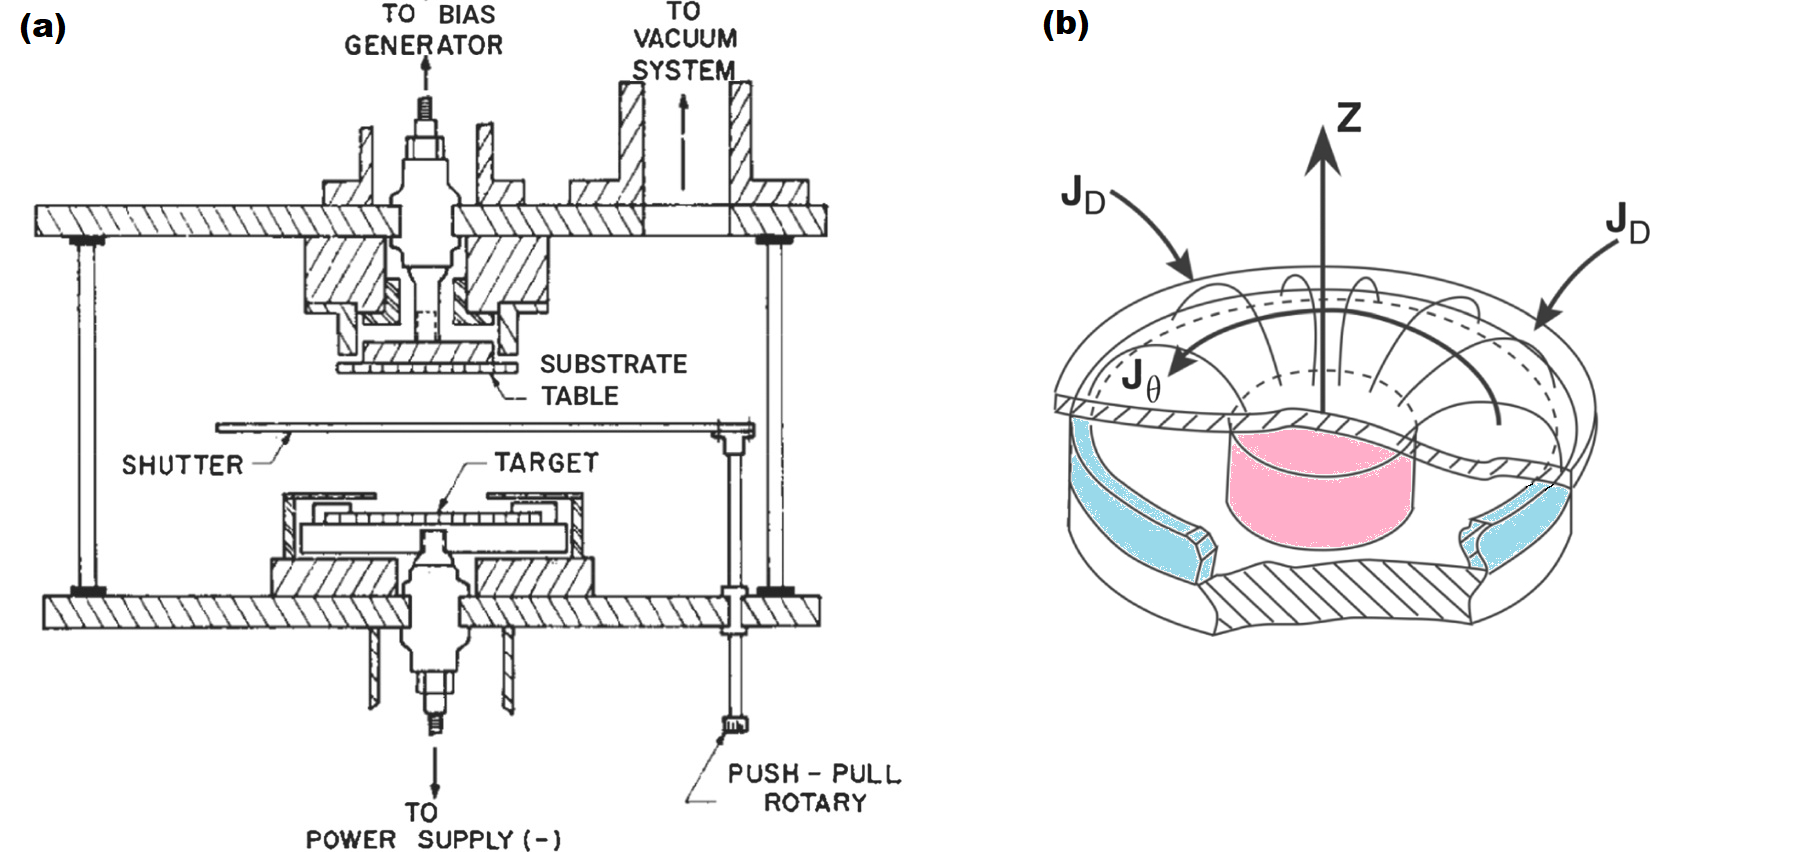
\includegraphics[width=0.8\textwidth]{figures/magnetron.png}
	\caption[Schematics of a magnetron sputtering system]{Schematics of a magnetron sputtering system (a) with cathode target (b). The plasma is confined by the magnetic field in a toroidal pattern\cite{songHandbookTerahertzTechnologies2015}.}\label{fig: magnetron}
\end{figure}